\begin{landscape}
\begin{figure}
    \centering
    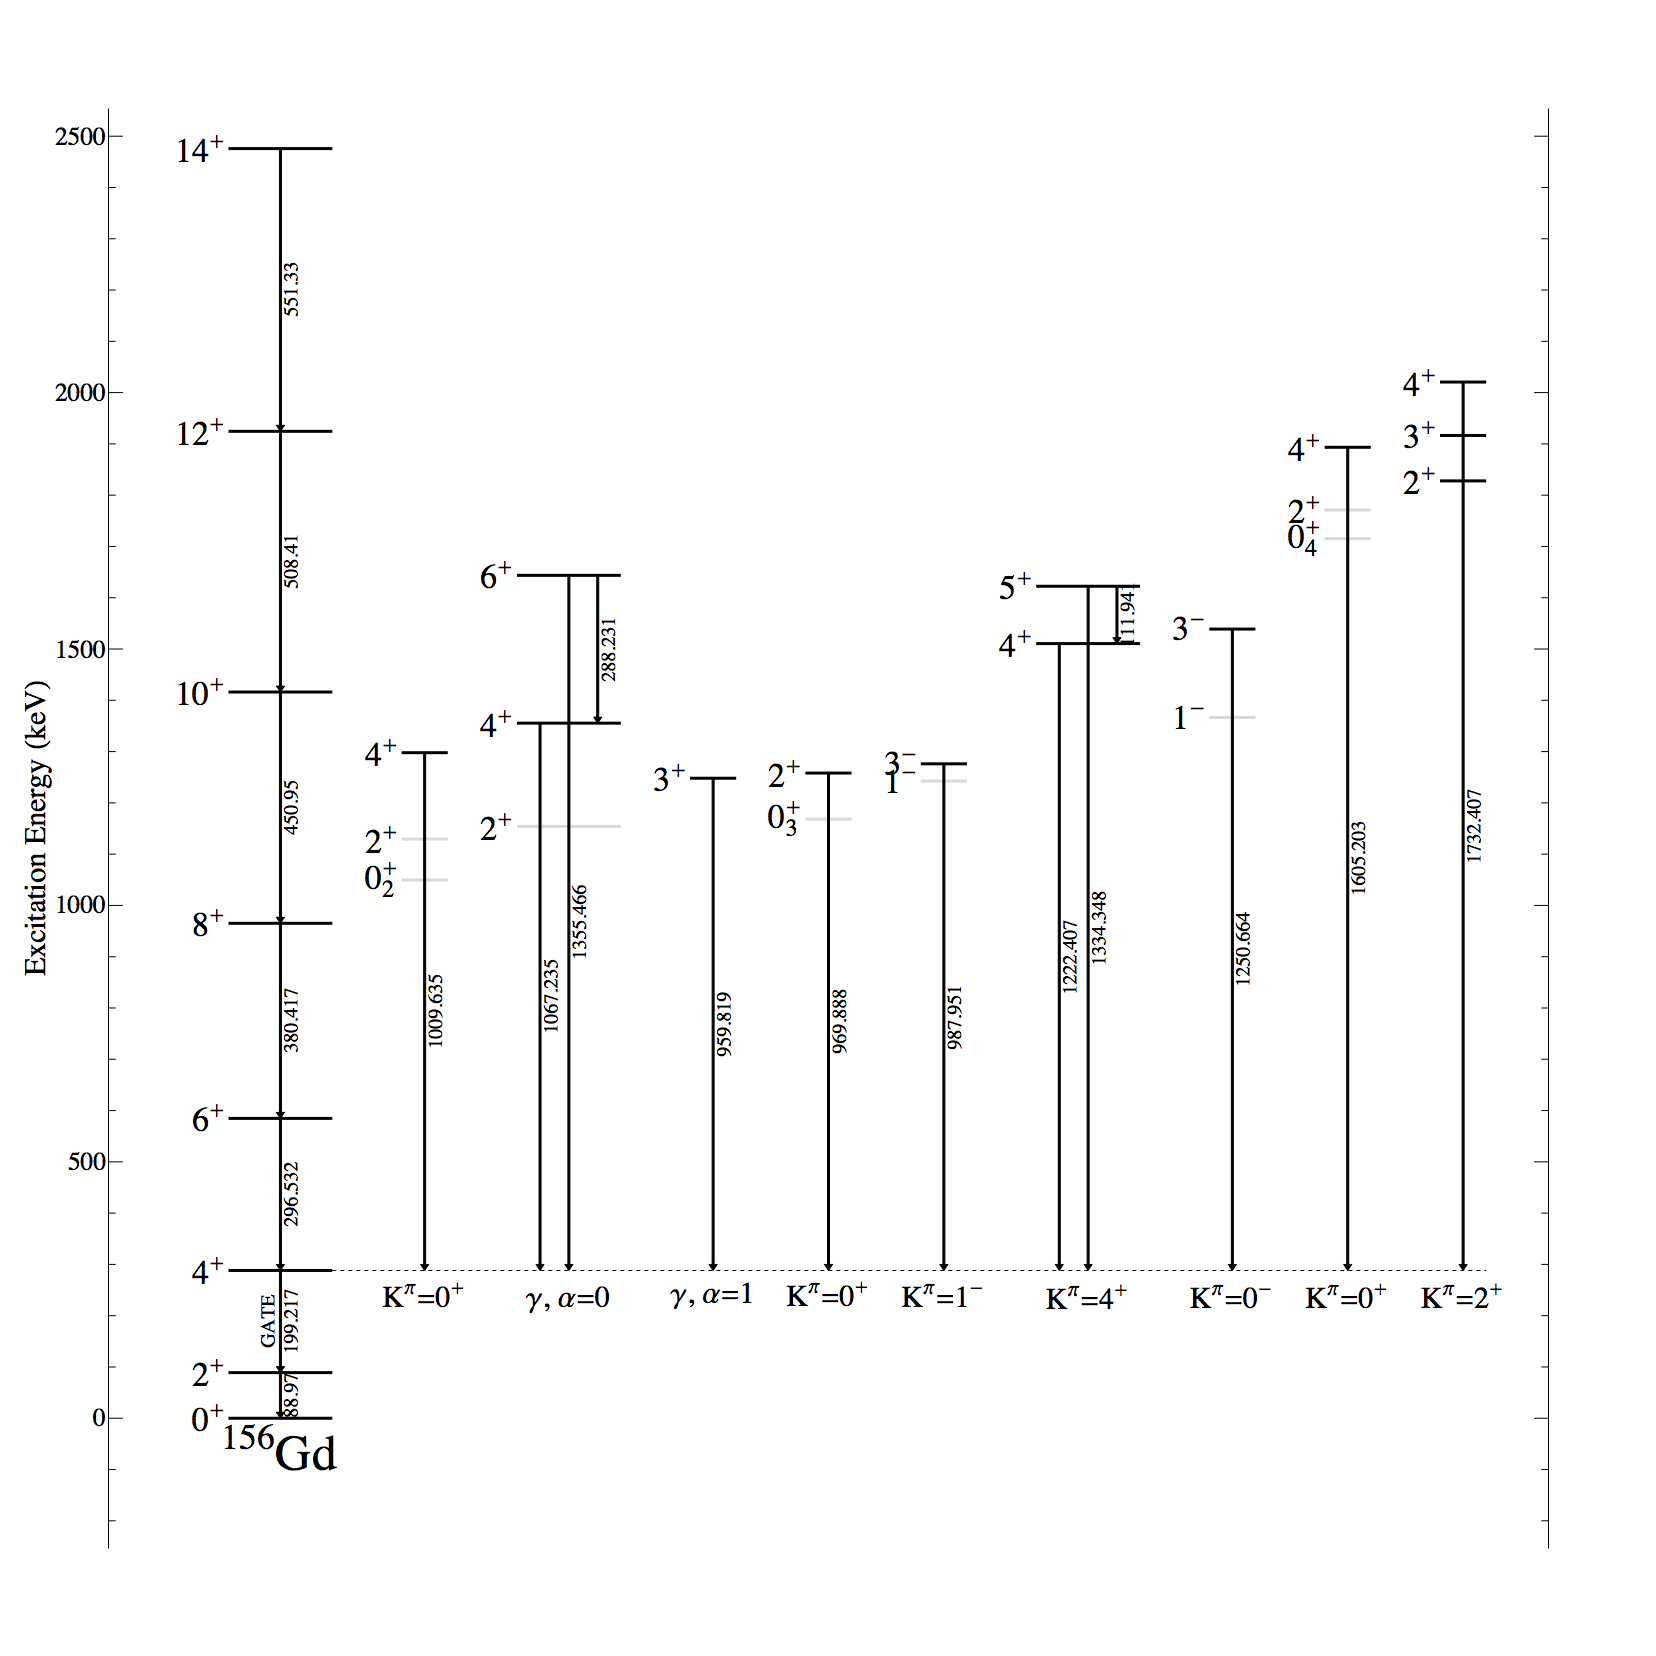
\includegraphics[scale=0.4]{156GdTablesAndFigs/156Gd_4to2.eps}
    \caption{Level Scheme of $^{156}$Gd. The gamma ray of the $4^+$\rightarrow$2^+$ (199 keV) transition in the ground state was gated on. It was then compared with the gated spectrum from the gamma ray of the $6^+$\rightarrow$4^+$ (296 keV) transition in the ground state. Peaks only appearing in the first gate were assumed to go into the $4^+$ state, and assignments were made. Additionally, these peaks were also gated on, to look for cascades leading into the $4^+$ state, which were found in several cases. The levels are organized by band. The lower levels of the band, unseen by gamma rays in this gate, are in gray.}
    \label{fig:156_4to2}
\end{figure}
\end{landscape}